\startchapter{Methods} \label{ch:2}
\section{Current approaches to molecular structure elucidation}
Currently, there are two main approaches in studying the orientation distribution of molecules at interface. One is comparing the experimental spectra with few predicted one, and select the one that most matches to the experimental one. Another one is running an exhaustive algorithm to explore the most possible solution space. \cite{hore0033-rotations}  However, both approaches take a lot of time and computational resources. In Hung's study \cite{KuoKaiHung:Thesis:2015}, a new approach is introduced by applying Linear Programming to vibrational spectra to extract the molecular structure elucidation. This LP approach helped to return the target orientation distribution information when the mock experimental spectrum consisted of different amino acids. However, when candidates are coming from the same amino acid, LP approach fail to return the target orientation distribution information. The reason why LP failed to return the target composition has not been thoroughly studied in Hung's study. My study is to figure out the underlying reason causing the return composition of the LP model does not match to the target composition. After this reason is resolved, we want to explore the limitation of the LP model. For the cases that LP model helps to return the target composition, we want to know if the LP models can be applied systematically to similar cases. \\
	
\section{Structure of molecules adsorbed to interfaces}
(TODO: check with Dennis, how to expand this part.) A picture to display molecules adsorbed to interfaces


\section{Generating model spectra}
As mentioned in Chapter \ref{ch:1}, before analyzing the vibrational spectra of amino acids, there are a few factors to address first. First of all, creating candidate spectra is an essential step. This part of research has been done thoroughly by Hung \cite{KuoKaiHung:Thesis:2015}. \\

To generate these amino acids' vibrational spectra, a molecule's vibration modes need to be modelled in the molecular frame, then transferred to the laboratory frame to work with the systems where interfaces exist. Chapter 2 in Hung's thesis \cite{KuoKaiHung:Thesis:2015} describes how to perform electronic structure calculations using GAMESS \cite{GAMESS} to obtain every dipole moment and polarizability derivatives. Then he introduced how to use Direction Cosine Matrix (DCM) to transfer these two derivatives from the molecular coordinate system to laboratory one. After that, Euler angles could be extracted from DCM. Euler angles are used to describe a molecule's coordination at interfaces. They are labelled by $\theta$, $\phi$ and $\psi$ as shown in Figure \ref{fig:2.1}, and referred as $tilt$, $azimuthal$ and $twist$ angles respectively. Let $x$, $y$ and $z$ be lab frame Cartesian coordinates, and $a$, $b$ and $c$ be the molecular frame coordinates. $Tilt$ angle $\theta$ is the angle between $z$ and $c$; $azimuthal$ angle $\phi$ is the rotation about $z$; and $twist$ angle $\psi$ is a twist about $c$ \cite{hore0033-rotations}. After three steps of successive rotations of Euler angles, molecule properties can be transferred from the molecular frame to the lab frame. \\


Hung first did a Hessian calculation. Secondly, 7 snapshots of a molecule vibrating in different modes were taken. Thirdly, he obtained the derivatives of dipole moment and polarizability based on these 7 modes' interpolation. Because the two obtained derivatives are in the molecular frame, Hung then used DCM to convert them into the lab frame.  Then abstracted Euler angles from DCM. After this transformation, he restored the derivatives information into some molecular property files for any further use. \\

\begin{figure}[!ht] \label{fig:2.1}
\centering
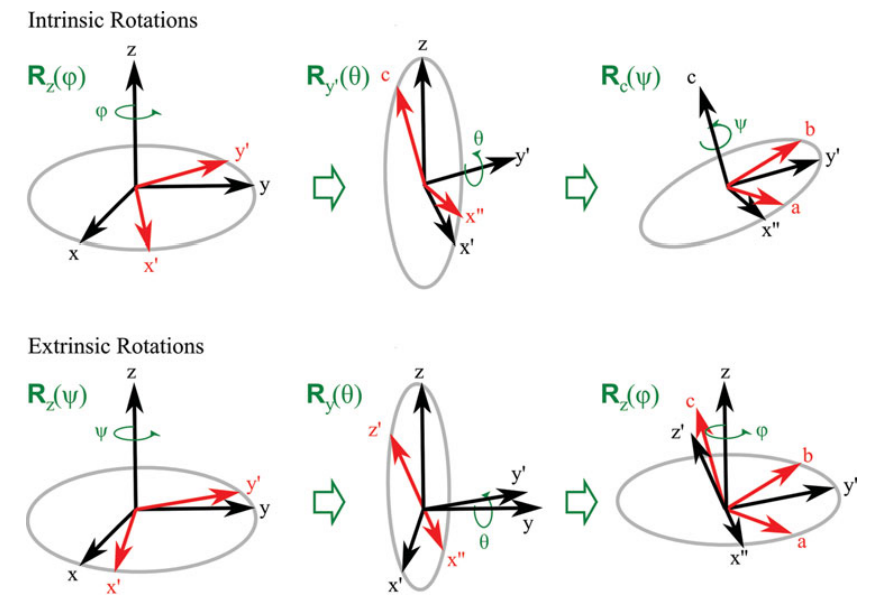
\includegraphics[scale=0.5]{Figures/Euler_angles_represented_as_the_spherical_polar_angles.png} 
\caption{The Euler angles represented as the spherical polar angles $\theta$, $\phi$ and $\psi$, and the illustration of the three successive rotations that transform the lab $x$, $y$, $z$ coordinate system into the molecular $a$, $b$, $c$ frame. \cite{RotationProjection}} 
\end{figure}

In my study, those molecular property files are used to generate the following amino acids' spectroscopy information: methionine, leucine, isoleucine, alanine, threonine and valine. Each molecular property file contains the derivatives of dipole moment and polarizabilities of vibrational mode of $3N-6$. $N$ is the number of atoms of a molecule. Furthermore, the following formulations \ref{eq:2.1} and \ref{eq:2.3} are used to generate each amino acid's IR, Raman and SFG spectra. \\

When molecules lay on an interface, the orientation for each molecule varies. This variety requires either do a molecular dynamic simulation to study the distribution of molecule orientations at the interface, or come up with a analytic orientation distribution function. In my study, the second method is preferred. Delta distribution function is used to represent the molecule orientation distribution that models the spectrum signals. \\

Furthermore, the experiments are limited to only consider the $tilt$ angle distribution of Euler angles, and assume isotropy in $twist$ and $azimuthal$ angular distributions. Therefore, these two Euler angles are integrated to create a uniform distribution for them. For angle $\psi$, it requires the surfaces to be not striped. However, there can be no anisotropy in the plane of the surface. Because of this, we limit the candidate number by integrating angle $\psi$. On the other hand, for angle $\phi$, a uniform distribution implies that the molecule has cylindrical symmetry in its preference of surface. This means that the molecule can be tilted, but has no `twist' preference. With the integration of these two Euler angles, the number of candidates for one molecule will be greatly reduced. However, the number is still large when only considering angle $\theta$. The possible combinations of all these amino acid candidates are still considered to be excessive (TODO: put these into an approximated number). \\

Infrared (IR) absorption spectroscopy is a harmonic approximation, its intensity is proportional to the square of the lab-frame dipole moment derivative. For example, the $x$-polarized absorption spectrum is given by Equation \ref{eq:2.1}. \\

\begin{equation} \label{eq:2.1}
I_x(\omega_{\rm IR}) = \sum_{q} \frac{1}{2 m_{q} w_{q}} \Bigg \langle \Bigg\lbrack \frac{\partial u_x}{\partial Q} \Bigg\rbrack_{q} ^2 \Bigg\rangle \frac{\Gamma_q^2}{(\omega_{\rm IR}-w_q)^2 + \Gamma_q^2}
\end{equation} 
where $I_x$ represents $x$-polarized intensity. The same equation applies to $I_y$ and $I_z$. $\omega_{\rm IR}$ is the frequency of the probe radiation. $\mu$ is the dipole moment. $m_q$ is the reduced mass. $w_q$ is resonance frequency. $\Gamma_q$ is the homogeneous line width, is set to 6 in all the experiments. $Q_q$ is the normal mode coordinate of the $q$th vibrational mode. All values of $\omega_{\rm IR}$, $\mu$, $m_q$, $Q$ are obtained from the molecular property files. Furthermore, because $\phi$ and $\psi$ angles are integrated, the $y$-polarized spectrum is identical with the $z$-polarized one. Therefore, in current experiments, only two different polarized IR spectra are obtained for one molecule. (TODO: need to double check the accuracy with Dennis)\\

%\begin{equation} \label{eq:2.1}
%I_x(w_{IR}) = \sum_{q} \frac{1}{2f m_{q} w_{q}} \Bigg \langle \Bigg\lbrack \frac{\partial u_x}{\partial Q} \Bigg\rbrack_{q} ^2 \Bigg\rangle \frac{\Gamma_q^2}{(w_{IR}-w_q)^2 + \Gamma_q^2}
%$f$ is the scaling factor for vibrational frequency, in experiemnt, this value swift a bit
%\end{equation} 


The intensity of Raman scattering is proportional to the square of laboratory-frame transition polarizability. For example, Raman spectroscopy with an $x$-polarized excitation source collects the $x$-polarized component of the scattered radiation, which can be approximated from Equation \ref{eq:2.2}. \\

\begin{equation} \label{eq:2.2}
I_{xx}(\Delta w) = \sum_{q} \frac{1}{2 m_{q} w_{q}} \Bigg \langle \Bigg\lbrack \frac{\partial \alpha_{xx}^{(1)}}{\partial Q} \Bigg\rbrack_{q} ^2 \Bigg\rangle \frac{\Gamma_q^2}{(\Delta w-w_q)^2 + \Gamma_q^2}
\end{equation} 
where $\Delta w$ is the Stokes Raman shift. $\alpha_{xx}^{(1)}$ is one component of the 9-element polarizability tensor. $m_q$, $w_q$, $\Gamma_q$, and $Q_q$ are the same as defined above for IR spectra. All the values of $\omega_{\rm IR}$, $\mu$, $m_q$, $Q$ are obtained from the molecular property files. Similar to IR spectroscopy, because of the integration of $\phi$ and $\psi$ angles, only 4 unique spectra are obtained from the following polarization: $xx$, $xy$, $xz$ and $zz$.  (TODO: double check the accuracy of the content with Dennis). \\

The intensity of SFG spectroscopy is proportional to the squared magnitude of the second-order susceptibility, $\left|  \chi^{(2)}\right|^{2}$. $\chi^{(2)}$ is derived from the second-order polarizability, $\alpha^{2}$.
's response intensity is governed by Equation \ref{eq:2.3}. \\
\begin{equation} \label{eq:2.3}
I_{xxx}(\omega_{\rm IR}) = \sum_{q} \frac{1}{2 m_{q} w_{q}} \Bigg \langle \Bigg\lbrack \frac{\partial \alpha_{xx}^{(1)}}{\partial Q} \Bigg\rbrack_{q} \Bigg\lbrack \frac{\partial u_{x}}{\partial Q} \Bigg\rbrack_{q} \Bigg\rangle \frac{1}{w_{q}-w_{IR}-i\Gamma_q}
\end{equation} 
where $I_{xxx}$ is the second-order susceptibility tensor. It is probed by an $x$-polarized visible incoming beam at frequency $w_{vis}$ and a $x$-polarized infrared beam incoming with frequency $w_{IR}$ are incident to the sample. Then the $x$-component of SFG at frequency $w_{SFG}=w_{vis}+w_{IR}$ is selected for detection. As $i=\sqrt{-1}$ is in the denominator, $X^{(2)}$ is a complex value \cite{KuoKaiHung:Thesis:2015}. The SFG response is the imaginary component of the second-order susceptibility. As in IR and Raman spectroscopy, all the values of $\omega_{\rm IR}$, $\mu$, $m_q$, $Q$ are obtained from the pickle files. Because of the integration of $\phi$ and $\psi$ angles, only 3 unique spectra are obtained from the following polarization: $yyz$, $yzy$ and $zzz$. (TODO: double check the accuracy of the content with Dennis). \\

With these equations and the pickle files, IR, Raman and SFG spectra can be generated for a specific molecule with certain Euler angles. In this study, only angle $\theta$ is considered. Therefore, only amino acid and its $\theta$ angle value needed to be specified. These three types of spectral information for a targeted candidate is generated. A candidate here is a specific amino acid (or molecule) with specific Euler angles (orientation at interfaces). (TODO: check accuracy with Dennis). \\

In Figure \ref{fig:2.2}, $x$-polarized IR spectra are for Methionine of the following values of $\theta$: $0^{\circ}$, $20^{\circ}$, $40^{\circ}$ and $60^{\circ}$. Their spectra are prefixed with $candidate\_$ in the labels. $ir\_x\_$ indicates the spectroscopy technique, ``number" indicates the $\theta$ angle's value. The spectra labelled as $target\_ir\_x$, is generated by combining $10\%$ of $candidate\_ir\_x\_0$, $50\%$ $candidate\_ir\_x\_20$ and $40\%$ $candidate\_ir\_x\_40$. (TODO: double check this sentence: "Putting the target spectra here is for comparing and visual")  \\

Similarly, Figure \ref{fig:2.3}, \ref{fig:2.4} and \ref{fig:2.5} depict the spectra of the same candidates and targets for $z$-polarized IR, $xx$-projection Raman and $yyz$-projection SFG spectrum respectively. For example in Figure \ref{fig:2.2}, the difference among the four candidates is significant. The biggest differences between exist at each vibrational mode. A valid wavenumber has values from 1000 to 2000. Therefore, for each projection, no matter IR, Raman or SFG is used. There are 200 data points can be extracted in the interval of 5 wavenumber (This also proved to be most effective experimentally as well).  With these data points, the corresponding LP model is contructed as described in Chapter \ref{ch:3}.\\

\begin{figure}[!ht]
\centering
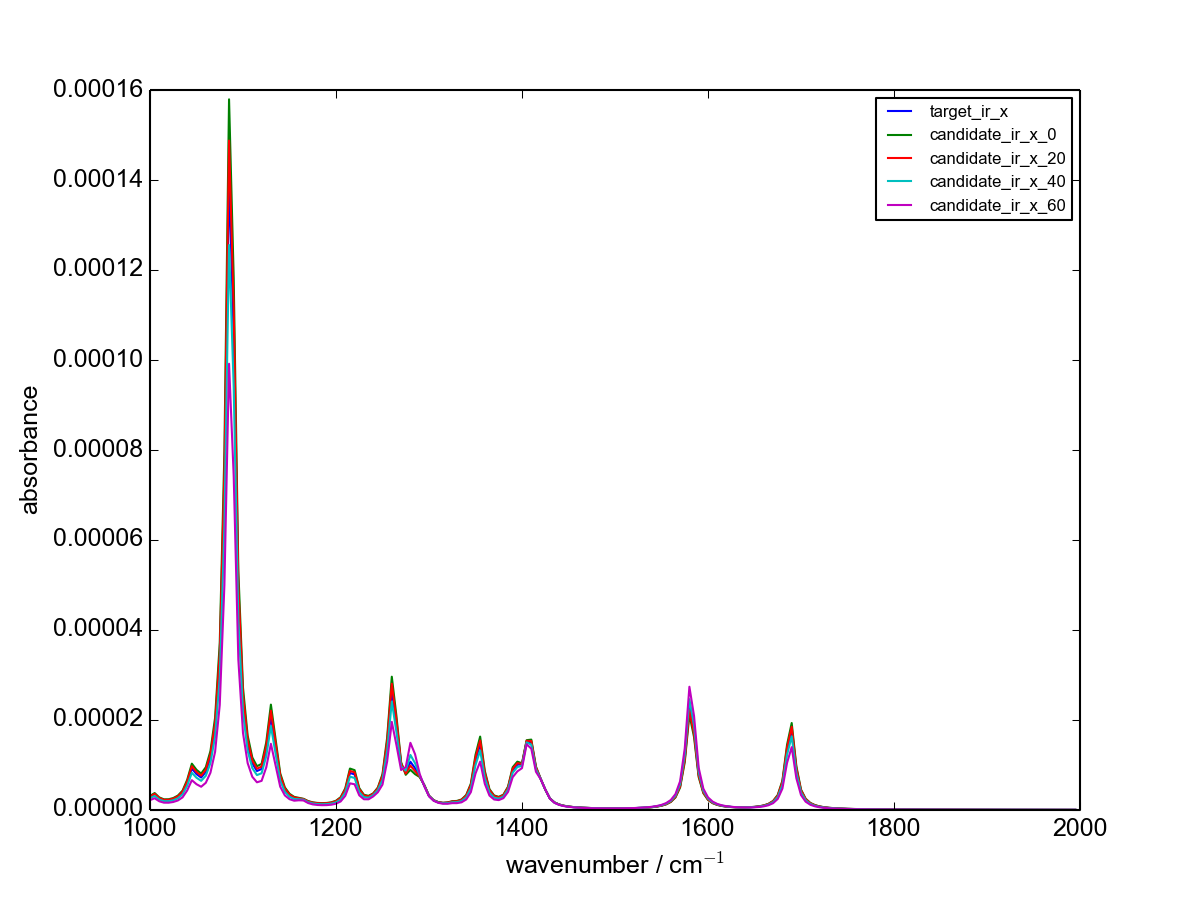
\includegraphics[scale=0.5]{Figures/Met_candidates_plotting_ir_x.png}
\caption{IR $x$ projection spectra for methionine four candidates and target} \label{fig:2.2}
\end{figure}

\begin{figure}[!ht]
\centering
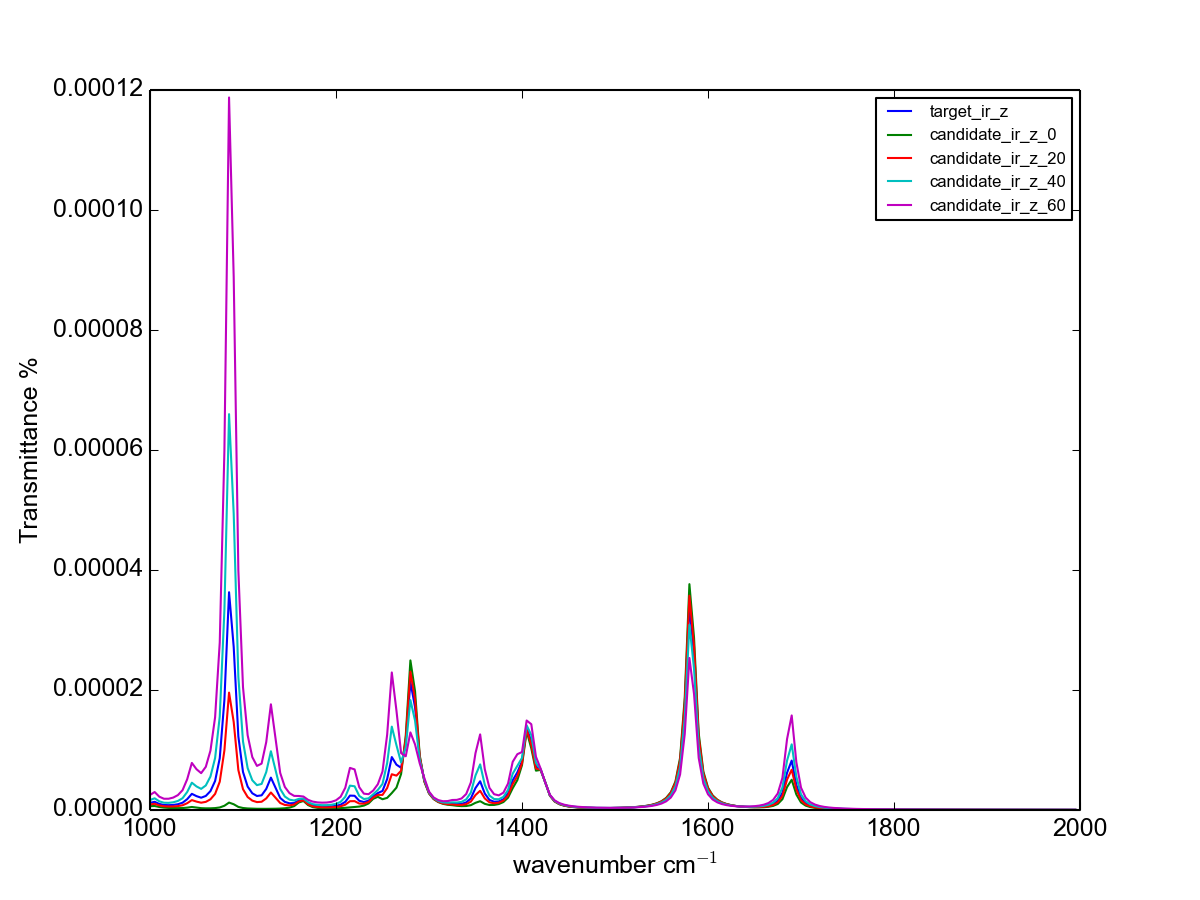
\includegraphics[scale=0.5]{Figures/Met_candidates_plotting_ir_z.png}
\caption{IR $z$ projection spectra for methionine four candidates and target} \label{fig:2.3}
\end{figure}

\begin{figure}[!ht]
\centering
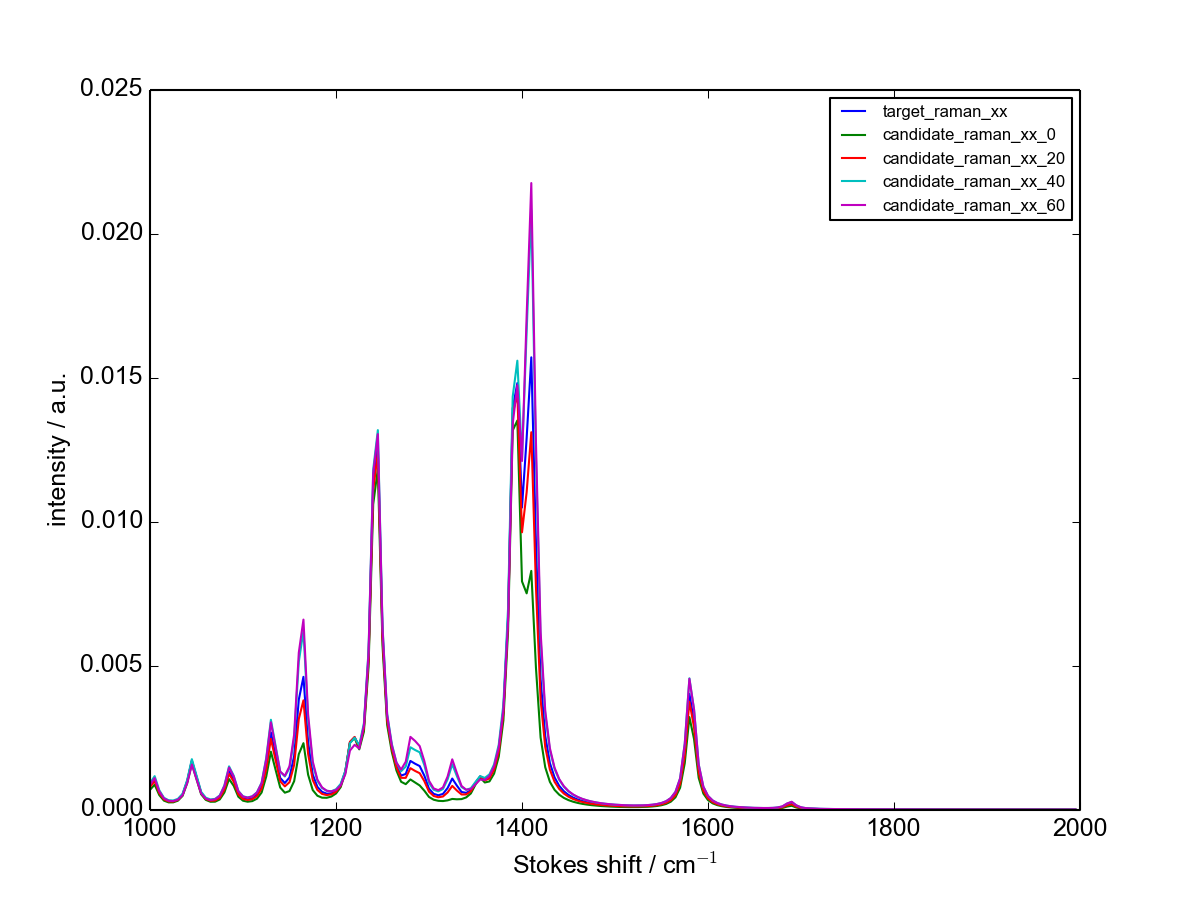
\includegraphics[scale=0.5]{Figures/Met_candidates_plotting_raman_xx.png}
\caption{Raman $xx$ projection spectra for methionine four candidates and target} \label{fig:2.4}
\end{figure}

\begin{figure}[!ht]
\centering
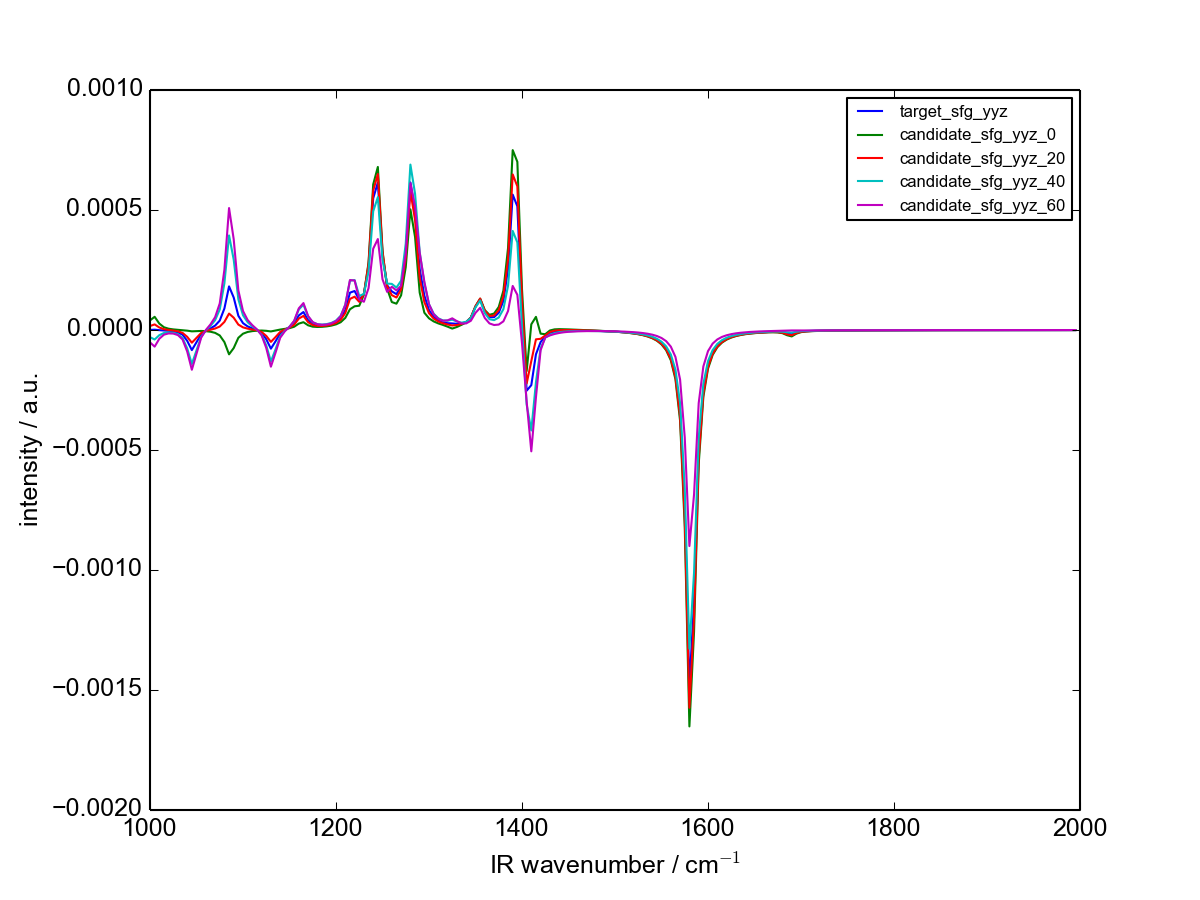
\includegraphics[scale=0.5]{Figures/Met_candidates_plotting_sfg_yyz.png}
\caption{SFG $yyz$ projection spectra for methionine four candidates and target} \label{fig:2.5}
\end{figure}


\section{Surface orientation distribution functions} 
(TODO: check with Dennis, how to expand this part.)





\section{The properties of the LP models}

In Chapter \ref{ch:3}, the properties of the LP models is studied. It is important to study the maximum capacity of the constructed LP models, and figure out what are the reasons that cause the limitation of them. Meanwhile, comparing the sensitivity of different spectroscopy techniques in the term of studying molecular orientation distribution at interfaces is also desired.

In order to achieve above goals, the properties of the LP models are studied first. In Chapter \ref{ch:3}, this part of study is conducted by using a toy model to gain an insight into the limitation of our LP approach. With the further information gained in Chapter \ref{ch:3}, further experiences will be conducted accordingly in Chapter \ref{ch:4}, \ref{ch:5} and \ref{ch:6}.

%Any spectroscopy data we obtain is in molecular frame, Cartesian coordinates like a, b, c. We have to convert it to lab frame(x, y, z) in order to describe molecular orientation. Therefore, we need to transfer molecule's main properties such as dipole moments and polarizability derivatives from molecular frame(a, b, c) to lab frame by Euler angles($\theta$, $\phi$, $\psi$). These three angles are parameters coming from Euler's rotation theorem that an arbitrary rotation can be parameterized by using three parameters. They are defined as Euler angles. Based on this theorem we know this transformation can be done through the 3D rotation matrix, which is direction cosine matrix(DCM) by Eq. 1.1.
%\begin{equation}
%	D=
%	\begin{pmatrix}
%	\cos\xi_{xa} & \cos\xi_{xb} & \cos\xi_{xc}\\
%	\cos\xi_{ya} & \cos\xi_{yb} & \cos\xi_{yc}\\
%	\cos\xi_{za} & \cos\xi_{zb} & \cos\xi_{zc}
%	\end{pmatrix}
%\end{equation}

%How to generate the candidates?

%Before we process our experiments, we need to generate all the amino acids candidates' spectra. In order to do that, we need obtain the properties of a molecule's vibrational modes in molecular frame first. And for all the amino acid molecules, we assume the orientation average adsorbed onto the surface based on mathematical distribution function, which is (Delta or Gaussian???) distribution in this case. Every molecule is made of atoms, and an atom contain protons, neutrons and electrons. Electrons play an important part in chemical reaction, by losing or gaining electrons, atoms bind to each other to construct a molecule. In an atom, electron is moving constantly, which makes a molecule having different electronic structures and different energy form. As a result, a molecule's dipole moment and polarizability are resided, and are changing all the time. \\

%The derivatives of dipole moment and polarizability is obtained by Kuo Kai Hung's previous work by using GAMESS\cite{[71]}. He did an hessian calculation first, then took 7 snapshots of molecule vibrating in different modes. And obtained the directives based on these 7 modes' interpolation. These two directive we obtained are in GAMESS's coordinate system (molecular frame), which is different from the interface (laboratory frame) that we want to study. Therefore, we need to convert the information from molecular frame to lab frame. In Kai's thesis, this coordinate transformation used direction cosine matrix(DCM) that described in Chapter 1, and then abstracted Euler angles from DCM. After transformation, the derivatives information is stored in pickle files for further usage.\\

%For our study, we are going to use the pickle files that include derivatives information of the following amino acids respectively: methionine, leucine, isoleucine, alanine, threonine and valine. For each pickle file, it contains derivatives of dipole moment and polarizabilities of mode from $0$ to $36$. We use the following formulations to develop IR, Raman and SFG spectrum.

%1. What are the pickle files?(put this part after spectroscopy techniques explaination)\\
%The pickle files that I am studying contain the dipole/polarizability properties information of the following Amino acids: Ala, Ile, Leu, Methionine, Thr, Val and Lys. (Refer to Kai's thesis about how these pickle files are generated). Take the pickle file that contains Methionine information as an example, from starting mode 0 to ending mode 36, the information about the deriviative of dipole moment and polarizabilities for each mode is obtained. \\

%2.What are the formulations we used to develop IR, Ramam and SFG spectrum? (The part is same as Kai's paper, should change? how?) \\